%!TEX root = ../../thesis.tex

\section{Feature Encoding}
\label{methodology:feature_encoding}

The feature encoding section of FlatCityBuf is responsible for the binary representation of 3D city objects and their associated data. This component preserves the semantic richness of the CityJSON model while leveraging FlatBuffers' efficient binary serialisation. The full schema definition for feature encoding can be found in \autoref{appendix:flatcitybuf_schema:feature}.

\subsection{CityFeature and CityObject Structure}
\label{methodology:feature_encoding:cityfeature_cityobject_structure}

FlatCityBuf implements the core structure of \ac{cjseq} using the following FlatBuffers tables:

\begin{itemize}
  \item \textbf{CityFeature} - \textit{table (root object)} - The top-level container for city objects:
    \begin{itemize}
      \item \textit{id} - Required string identifier, marked as a key field for fast lookup
      \item \textit{objects} - Array of CityObject tables representing individual 3D features
      \item \textit{vertices} - Array of Vertex structs containing quantized X,Y,Z coordinates (int32)
      \item \textit{appearance} - Optional Appearance table with visual styling information
    \end{itemize}

  \item \textbf{CityObject} - \textit{table} - Individual 3D city objects:
    \begin{itemize}
      \item \textit{type} - CityObjectType enum (Building, Bridge, etc.) following CityJSON types \citep{cityjson_spec}
      \item \textit{id} - Required string identifier, marked as a key field
      \item \textit{geographical\_extent} - 3D bounding box as GeographicalExtent struct
      \item \textit{geometry} - Array of Geometry tables containing shape information
      \item \textit{attributes} - Binary blob containing attribute values (interpretable via columns schema)
      \item \textit{columns} - Array of Column tables defining attribute schema
      \item \textit{children} - Array of string IDs referencing child objects
      \item \textit{children\_roles} - Array of strings describing relationship roles
      \item \textit{parents} - Array of string IDs referencing parent objects
      \item \textit{extension\_type} - Optional string for extended object types (e.g., "+NoiseBuilding")
    \end{itemize}
\end{itemize}

This structure maintains CityJSON's hierarchical organization while taking advantage of FlatBuffers' binary encoding and zero-copy access capabilities. The one-to-many relationship between \ac{cityfeature} and CityObject enables efficient vertex sharing while preserving semantic distinctions between different city elements.

\subsection{Geometry Encoding}
\label{methodology:feature_encoding:geometry_encoding}

Geometry in FlatCityBuf follows CityJSON's boundary representation (B-rep) model with flattened arrays for FlatBuffers encoding:

\begin{itemize}
  \item \textbf{Geometry} - \textit{table} - Container for geometric representation:
    \begin{itemize}
      \item \textit{type} - GeometryType enum representing dimensions (0D-Point, 1D-LineString, etc.)
      \item \textit{lod} - Level of Detail as float value
      \item \textit{boundaries} - Array of 32-bit indices referencing vertices
      \item \textit{strings} - Array of counts defining vertex groups
      \item \textit{surfaces} - Array of counts defining string groups
      \item \textit{shells} - Array of counts defining surface groups
      \item \textit{solids} - Array of counts defining shell groups
      \item \textit{semantics\_boundaries} - Parallel arrays to boundaries for semantic classification
      \item \textit{semantics\_values} - Array of SemanticObject tables
    \end{itemize}

  \item \textbf{SemanticObject} - \textit{table} - Semantic classification of geometry parts:
    \begin{itemize}
      \item \textit{type} - SemanticSurfaceType enum (WallSurface, RoofSurface, etc.)
      \item \textit{extension\_type} - Optional string for extended semantic types
      \item \textit{attributes} - Binary blob containing semantic-specific attributes
      \item \textit{columns} - Array of Column tables defining attribute schema
      \item \textit{parent} - Index to parent semantic object
      \item \textit{children} - Array of indices to child semantic objects
    \end{itemize}

  \item \textbf{GeometryInstance} - \textit{table} - Reference to template geometry:
    \begin{itemize}
      \item \textit{transformation} - 4×4 transformation matrix as TransformationMatrix struct
      \item \textit{template} - Index referencing a template in the header section
      \item \textit{boundaries} - Single-element array containing reference point index
    \end{itemize}

  \item \textbf{Vertex} - \textit{struct} - Quantized 3D coordinates:
    \begin{itemize}
      \item \textit{x, y, z} - Integer coordinates, converted to global coordinates using header transform
    \end{itemize}
\end{itemize}

\subsubsection{Hierarchical Boundaries as Flattened Arrays}
\label{methodology:feature_encoding:geometry_encoding:flattened_arrays}

A key challenge in adapting CityJSON's recursive boundary representation to FlatBuffers is that FlatBuffers does not support nested arrays. FlatCityBuf addresses this by implementing a dimensional hierarchy encoded as parallel flattened arrays:

\todo{replace with proper figure}
\begin{figure}[htbp]
  \centering
  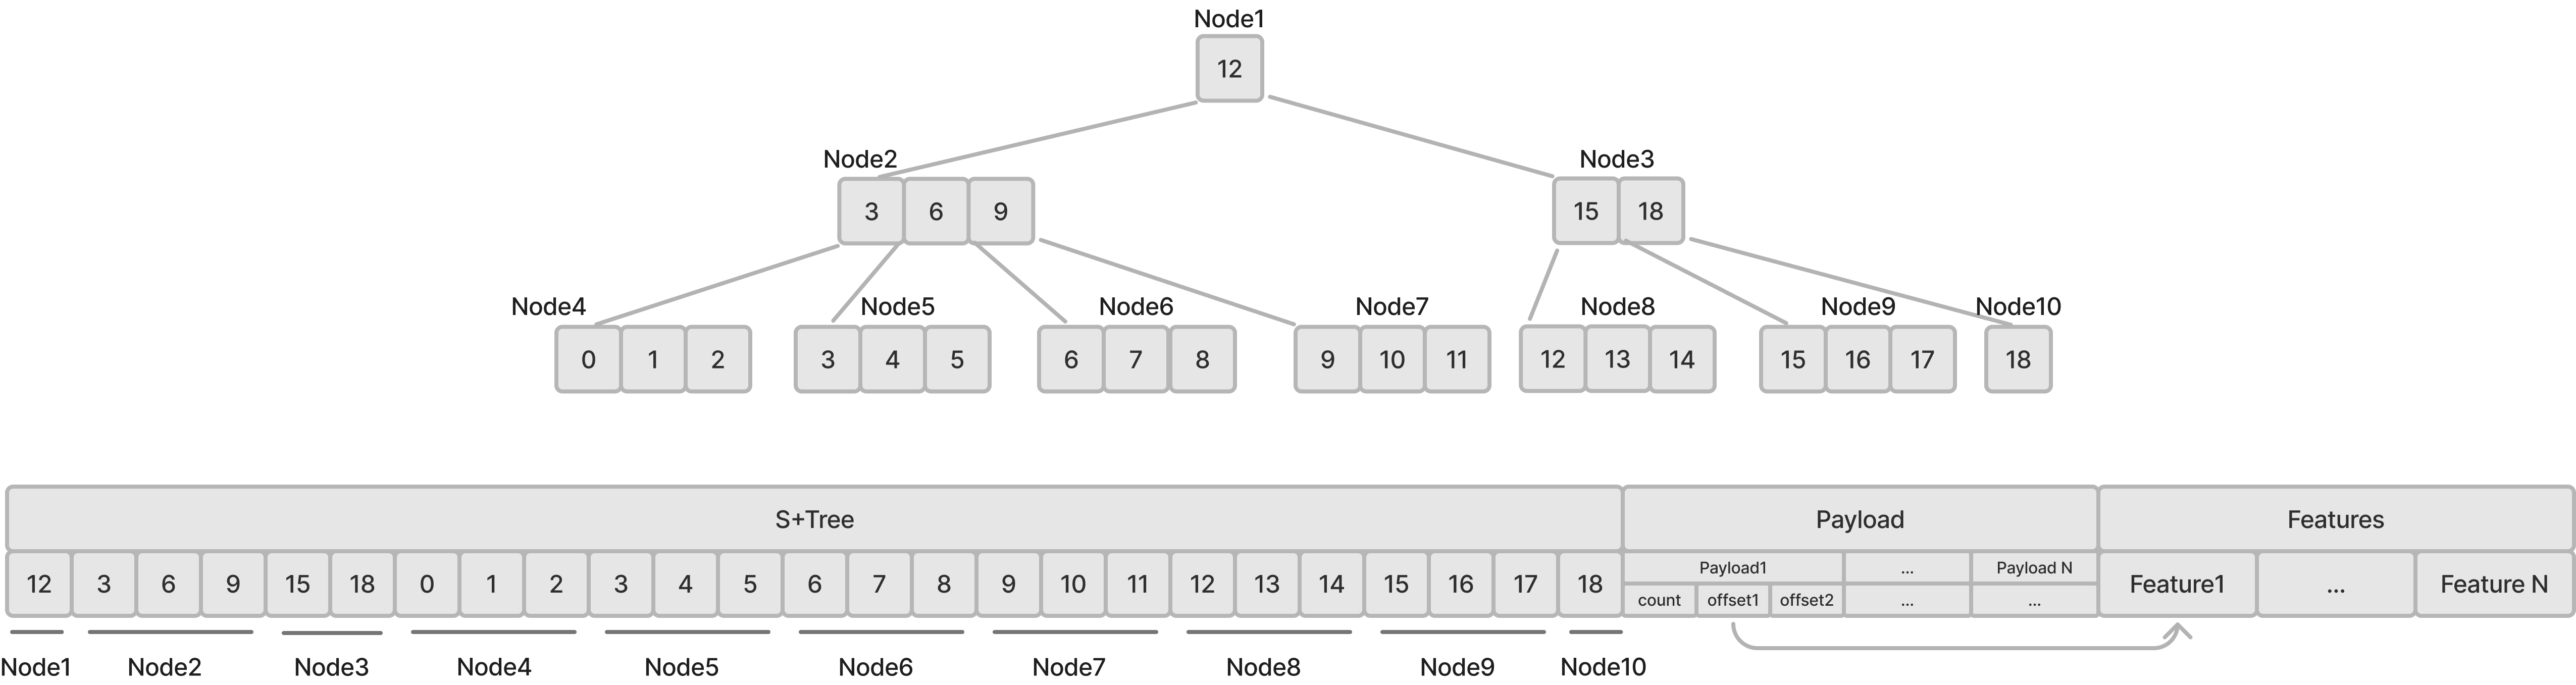
\includegraphics[width=0.8\textwidth]{figs/methodology/attribute_index.png}
  \caption{Hierarchical encoding of boundary representation using flattened arrays}
  \label{fig:methodology:boundary_encoding}
\end{figure}

The encoding strategy follows a dimensional hierarchy from lowest to highest dimension:

\begin{enumerate}
  \item \textbf{boundaries}: A single flattened array of integer vertex indices
  \item \textbf{strings}: Array where each value indicates the number of vertices in each ring/boundary
  \item \textbf{surfaces}: Array where each value indicates the number of strings/rings in each surface
  \item \textbf{shells}: Array where each value indicates the number of surfaces in each shell
  \item \textbf{solids}: Array where each value indicates the number of shells in each solid
\end{enumerate}

For example, a simple triangle would be encoded as:

\begin{verbatim}
boundaries: [0, 1, 2]       // Indices of three vertices
strings: [3]                // Single string with 3 vertices
surfaces: [1]               // Single surface containing 1 string
\end{verbatim}

A more complex structure such as a cube (a solid with 6 quadrilateral faces) would be encoded as:

\begin{verbatim}
boundaries: [0, 1, 2, 3, 0, 3, 7, 4, 1, 5, 6, 2, 4, 7, 6, 5, 0, 4, 5, 1, 2, 6, 7, 3]
strings: [4, 4, 4, 4, 4, 4]    // 6 strings with 4 vertices each
surfaces: [1, 1, 1, 1, 1, 1]   // 6 surfaces with 1 string each
shells: [6]                    // 1 shell with 6 surfaces
solids: [1]                    // 1 solid with 1 shell
\end{verbatim}

\subsubsection{Semantic Surface Encoding}
\label{methodology:feature_encoding:geometry_encoding:semantics}

Semantic surface information is encoded using a similar approach:

\begin{itemize}
  \item \textbf{semantics\_values}: Array of SemanticObject tables containing type classifications, attributes, and hierarchical relationships
  \item \textbf{semantics\_boundaries}: Array of indices that reference entries in semantics\_values, with a parallel structure to the geometry boundaries
\end{itemize}

This parallel structure allows each geometric component to have associated semantic information without requiring deeply nested structures. For example, in a building model where each face has a semantic classification (wall, roof, etc.), the semantics\_boundaries array would have the same structure as the boundaries array, with each surface having a corresponding semantic value.

Through this flattened array approach, FlatCityBuf preserves the rich hierarchical structure of CityJSON geometries while conforming to FlatBuffers' efficiency-oriented constraints on data organization.

\subsubsection{Geometry Template Encoding}
\label{methodology:feature_encoding:geometry_encoding:templates}

FlatCityBuf implements CityJSON's template mechanism for efficient representation of repeated geometry patterns, a common requirement in urban environments where many buildings, street furniture items, or other objects share identical geometric structures. The template approach separates the geometry definition from its instantiation:

\begin{itemize}
  \item \textbf{Template Definition}: Templates are defined once in the header section as full Geometry objects:
    \begin{itemize}
      \item Templates use the same Geometry table format described previously for standard geometries
      \item Template vertices are stored with double-precision coordinates (\texttt{DoubleVertex}) to maintain accuracy in the local coordinate system
      \item All template vertices for all templates are stored in a single flat array (\texttt{templates\_vertices})
      \item Indices within template boundaries reference positions in this dedicated template vertex array
    \end{itemize}

  \item \textbf{Template Instantiation}: CityObjects reference templates through GeometryInstance tables:
    \begin{itemize}
      \item \texttt{template}: A single unsigned integer index referencing a specific template in the header
      \item \texttt{boundaries}: Contains exactly one index referencing a vertex in the feature's vertex array, which serves as the reference point for placement
      \item \texttt{transformation}: A 4×4 transformation matrix (rotation, translation, scaling) that positions the template relative to the reference point
    \end{itemize}
\end{itemize}

This approach provides significant storage efficiency, as potentially complex geometries with hundreds or thousands of vertices can be represented using just a few bytes per instance. For example, a dataset with 1,000 identical street lamps would store the detailed lamp geometry once in the header, with each instance requiring only an index reference, reference point, and transformation matrix—typically less than 140 bytes per instance instead of potentially kilobytes of repeated geometry data.

The transformation matrix enables not only positioning but also scaling and rotation, allowing templates to be adapted to specific contexts. This is particularly valuable for features like trees, street furniture, or modular building components that maintain the same basic shape but may vary in size or orientation.

\subsection{Materials and Textures}
\label{methodology:feature_encoding:materials_textures}

FlatCityBuf supports CityJSON's appearance model through the following structures:

\begin{itemize}
  \item \textbf{Appearance} - \textit{table} - Container for visual styling information:
    \begin{itemize}
      \item \textit{materials} - Array of Material tables
      \item \textit{textures} - Array of Texture tables
      \item \textit{vertices\_texture} - Array of Vec2 structs for UV coordinates
      \item \textit{material\_mapping} - Array of MaterialMapping tables
      \item \textit{texture\_mapping} - Array of TextureMapping tables
      \item \textit{default\_theme\_material} - String identifying default material theme
      \item \textit{default\_theme\_texture} - String identifying default texture theme
    \end{itemize}

  \item \textbf{Material} - \textit{table} - Surface visual properties:
    \begin{itemize}
      \item \textit{name} - Required string identifier
      \item \textit{ambient\_intensity} - Double value from 0.0 to 1.0
      \item \textit{diffuse\_color} - Array of double values (RGB)
      \item \textit{emissive\_color} - Array of double values (RGB)
      \item \textit{specular\_color} - Array of double values (RGB)
      \item \textit{shininess} - Double value from 0.0 to 128.0
      \item \textit{transparency} - Double value from 0.0 to 1.0
      \item \textit{is\_smooth} - Boolean flag for smooth shading
    \end{itemize}

  \item \textbf{Texture} - \textit{table} - Image mapping information:
    \begin{itemize}
      \item \textit{type} - TextureFormat enum (PNG, JPG)
      \item \textit{image} - Required string containing image file name or URL
      \item \textit{wrap\_mode} - WrapMode enum (None, Wrap, Mirror, Clamp, Border)
      \item \textit{texture\_type} - TextureType enum (Unknown, Specific, Typical)
      \item \textit{border\_color} - Array of double values (RGBA)
    \end{itemize}

  \item \textbf{MaterialMapping} and \textbf{TextureMapping} - \textit{tables} - Link materials/textures to surfaces:
    \begin{itemize}
      \item \textit{theme} - String identifier for themes (e.g., "summer", "winter")
      \item \textit{values} - Indices to surfaces or boundaries
      \item \textit{material/texture} - Index to the referenced material or texture
    \end{itemize}
\end{itemize}

This implementation prioritizes efficient storage by referencing external texture files rather than embedding image data directly, enabling selective loading based on application requirements while maintaining full compatibility with CityJSON's appearance model.

\subsubsection{Texture Storage Design Rationale}
\label{methodology:feature_encoding:textures:rationale}

FlatCityBuf stores texture references rather than embedding texture data directly for several strategic reasons:

\begin{itemize}
  \item \textbf{Performance Priority}: Enables rapid loading of geometric and semantic data without the overhead of large texture files when not required.

  \item \textbf{On-demand Loading}: Supports selective texture loading based on application needs, beneficial for analysis-focused use cases.

  \item \textbf{Size Management}: Maintains reasonable file sizes for large-scale datasets, essential for spatial indexing operations.

  \item \textbf{Web Efficiency}: Aligns with HTTP caching mechanisms, optimizing repeated access in browser environments.
\end{itemize}

This approach follows established patterns in formats like glTF and I3S, prioritizing operational efficiency over self-contained packaging for city-scale datasets.

\subsection{Attribute Encoding}
\label{methodology:feature_encoding:attribute_encoding}

Attributes in FlatCityBuf are encoded as binary data with a schema defined through Column tables, which were detailed previously in \autoref{methodology:header:schema_indexing}. Rather than repeating column structure information, this section focuses on the binary encoding strategy:

\begin{itemize}
  \item \textbf{Attribute Binary Encoding} - Efficient type-specific serialization:
    \begin{itemize}
      \item \textit{Numeric types} - Native binary representation (little-endian)
      \item \textit{String} - Length-prefixed UTF-8 encoding
      \item \textit{Boolean} - Single byte (0 = false, 1 = true)
      \item \textit{Date/DateTime} - Standardized binary format
      \item \textit{Null} - Represented according to type (0, empty string, etc.)
    \end{itemize}
\end{itemize}

By encoding attributes as type-specific binary values with a corresponding schema, FlatCityBuf achieves significant storage efficiency compared to self-describing formats like JSON. The column-based approach also aligns with common database practices, facilitating integration with existing GIS and database systems. The figure below highlights the binary encoding process for different attribute types, demonstrating how the schema-driven approach reduces storage requirements while maintaining full data fidelity.

\todo{replace with proper figure}
\begin{figure}[htbp]
  \centering
  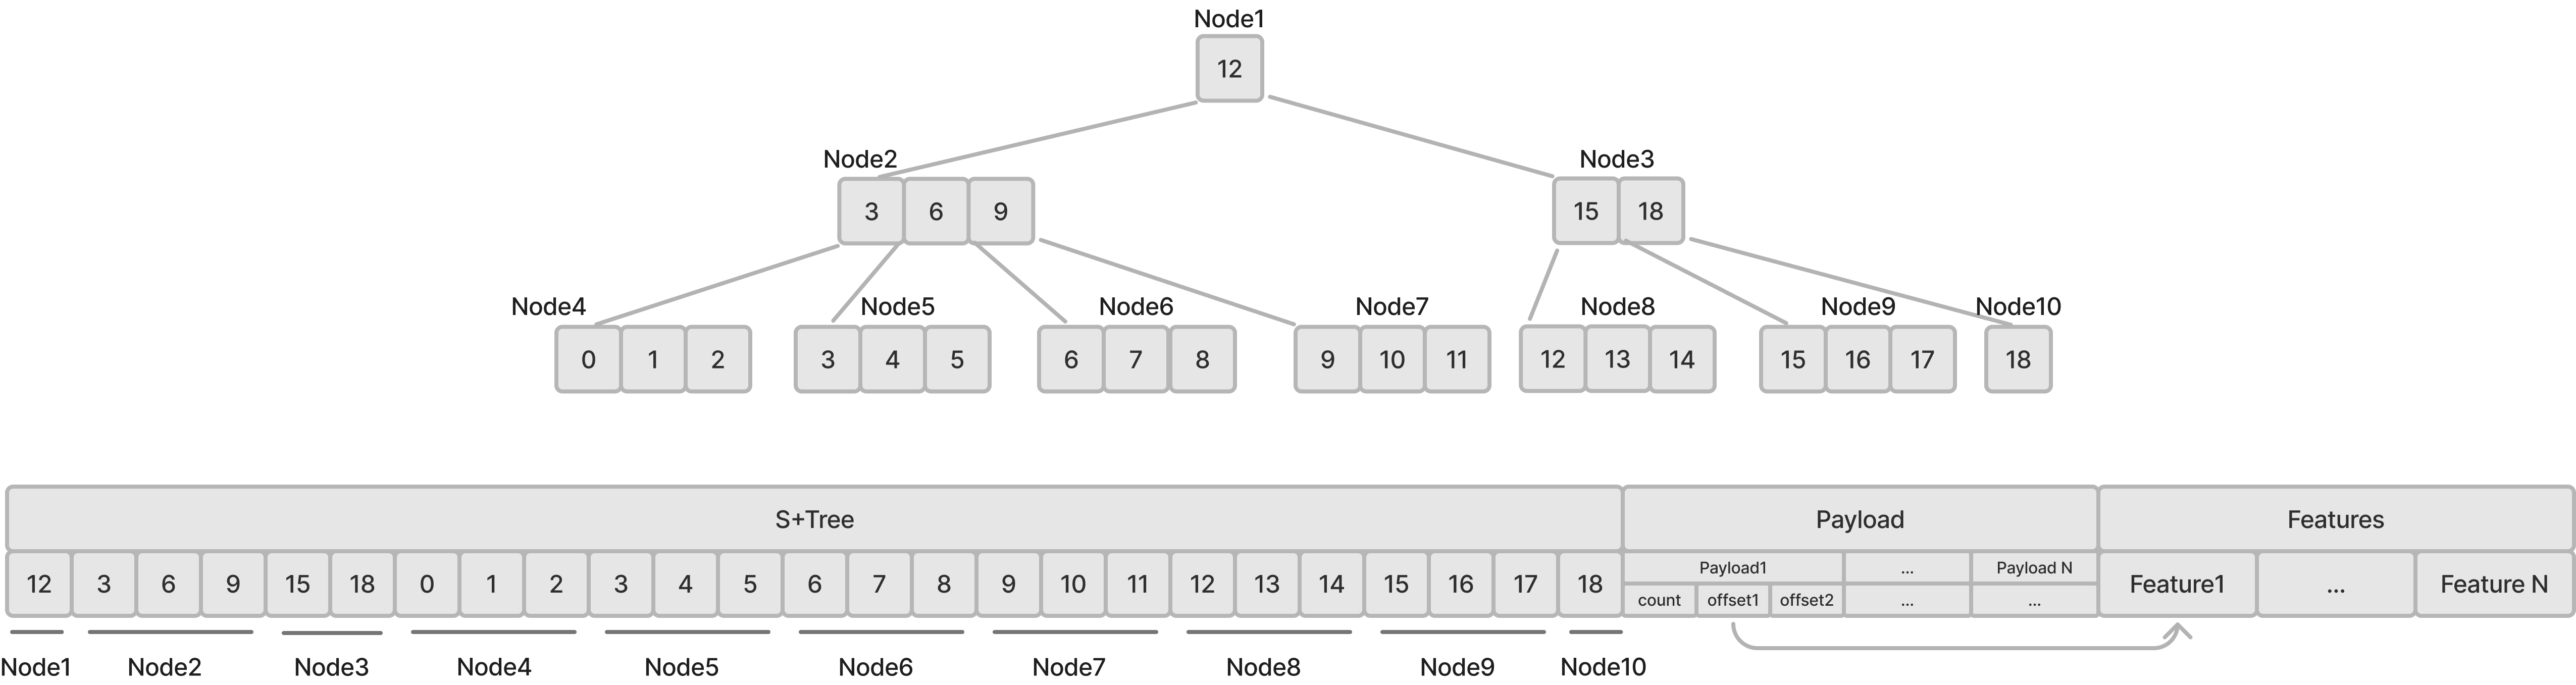
\includegraphics[width=0.8\textwidth]{figs/methodology/attribute_index.png}
  \caption{Attribute Encoding Process}
  \label{methodology:feature_encoding:attribute_encoding:figure}
\end{figure}

\subsection{Extension Mechanism}
\label{methodology:feature_encoding:extension_mechanism}

FlatCityBuf provides comprehensive support for CityJSON's extension mechanism, which was previously detailed in \autoref{methodology:header:extensions}. While the extension structures are defined in the header, their implementation within actual city features requires specific encoding strategies that balance extensibility with performance.

\subsubsection{Encoding of Extended City Objects}
\label{methodology:feature_encoding:extension_mechanism:city_objects}

Extended city object types (those prefixed with "+") are encoded using a two-part strategy:

\begin{itemize}
  \item A standard enum value \texttt{ExtensionObject} is used for the \texttt{type} field, providing efficient storage and processing
  \item The actual extension type name (e.g., "+NoiseCityFurnitureSegment") is stored in the \texttt{extension\_type} string field
\end{itemize}

This hybrid approach offers an optimal balance: the fixed enum value enables fast processing and type checking, while the string field preserves the full semantic information without requiring enum updates for new extension types.

\subsubsection{Encoding of Extended Semantic Surfaces}
\label{methodology:feature_encoding:extension_mechanism:semantic_surfaces}

Similarly, extended semantic surface types follow the same pattern:

\begin{itemize}
  \item The \texttt{type} field uses the enum value \texttt{ExtraSemanticSurface}
  \item The specific type (e.g., "+ThermalSurface") is stored in the \texttt{extension\_type} field
\end{itemize}

\subsubsection{Extension Attribute Encoding}
\label{methodology:feature_encoding:extension_mechanism:attributes}

Extension-specific attributes are encoded using the same binary serialization mechanism as core attributes:

\begin{itemize}
  \item Extension attributes are included in the same binary attribute blob as standard attributes
  \item The schema for these attributes is derived from the extension definition in the header
  \item No distinction is made at the storage level between core and extension attributes, simplifying implementation
\end{itemize}

During decoding:
\begin{itemize}
  \item If a CityObject has \texttt{type=ExtensionObject}, the application uses \texttt{extension\_type} to determine proper handling
  \item All attributes are decoded according to the provided schema, regardless of whether they belong to the core CityJSON specification or to an extension
\end{itemize}

Unlike CityJSON, which references external schema files for extensions, FlatCityBuf's self-contained approach ensures that all extension information is available within a single file. This approach maintains the cloud-optimized philosophy of minimizing external dependencies while preserving full compatibility with the rich extension capabilities of CityJSON.
